%!TEX root = ../../../thesis.tex

Details of components in the electrode-electrolyte interface model and methods of determining its parameters have been discussed.
Focus will now move to measuring and fitting suitable parameter values to the model.
Model parameters are determined for various concentrations of phosphate buffered saline (PBS), and then for comparison -- in a living sheep's spinal cavity.
The comparison will show whether a one-tenth concentration of PBS is in-fact a good substitute for cerebrospinal fluid (CSF), which it is assumed to be by medical implant engineers.

\section{Phosphate Buffered Saline}
\label{sect:pbs_measurements}

    Scott \& Single fitted parameters of their model to a one-tenth concentration (0.1X) of a standard solution of PBS.
    A one-tenth concentration of PBS is a commonly used solution of buffered saline \cite{Scott2014}.
    I measure and fit parameters not only to the one-tenth concentration, but to six concentrations spanning 0.025X to 1X the concentration of a standard buffered saline solution.
    For the model parameters that change with salinity, a fit is made using regression analysis to PBS concentration.
    Doing so provides a model that can be used to predict the impedance response of an electrode array submerged in a wider range of saline concentrations.

    Each of the PBS measurements were made in \SI{1000}{\milli\litre} glass bottles containing \SI{700}{\milli\litre} of the PBS solution to be measured.
    Measurements were made in a temperature controlled environment set at \SI{21}{\degree} Celsius.
    All measurements were automated by the use of Python scripts running on a GNU/Linux based workstation.
    The scripts communicate with the instruments both to configure measurements and collect data.
    Each measurement set was repeated for each of the six solutions used.
    The six concentration of PBS that were measured are shown in \cref{tab:pt2-PBS_concentrations}.
    \begin{table}
      \centering
      \begin{tabular}{l}
        Concentration\\
        \hline
        1.00X\\
        0.5X\\
        0.25X\\
        0.1X\\
        0.05X\\
        0.025X\\
      \end{tabular}
      \caption{\label{tab:pt2-PBS_concentrations}Six PBS concentrations used to fit model parameters to.}
    \end{table}

    % Edit checkpoint 2015-09-19 10:17


    \subsection{Inter-electrode resistivity}


      \begin{figure}
        \centering
        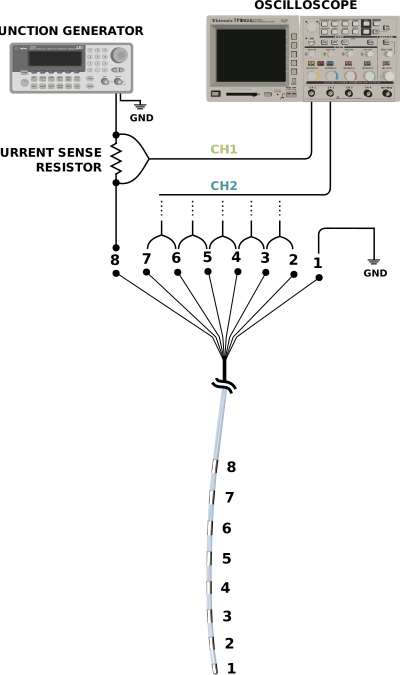
\includegraphics{content/pt2/08-InterfaceParameters/graphics/measurement_resistorMesh}
        \caption{\label{fig:pt2-measurement_resistorMesh}Illustration of one of two measurement configurations used to measure the electrode trans-impedances. Each of the electrode pairs were measured in sequence using the shown equipment.}
      \end{figure}

      With the electrode array immersed in a saline solution, a \SI{10}{\kilo\hertz} sinusoidal current having a peak amplitude of \SI{500}{\micro\ampere} was passed through the stimulus electrodes using an Agilent 33220A function generator.
      A shunt resistor inserted in series with the function generator allows measurement of current between electrodes.
      The differential voltage across a pair of non-stimulating electrodes and the voltage across the shunt resistor was measured using a Tektronix TPS 2024 oscilloscope.
      \Cref{fig:pt2-measurement_resistorMesh} shows the measurement configuration used when electrodes one and eight are used as the stimulus electrodes.
      The second configuration has electrodes eight and seven as stimulus electrodes and the remaining electrode pairs are used to measure trans-impedance voltage differentials.

      \begin{figure}
        \centering
        \includegraphics{content/pt2/07-InterfaceModel/graphics/graph_transimpedance_pbs}
        \caption{\label{fig:pt2-graph_transimpedance_pbs}Measured and fitted values of trans-impedance for both measurement configurations. Voltage measurements are made between adjacent pairs of electrodes as current is pushed through the stimulus electrodes.}
      \end{figure}
      The results of those measurements, in both configurations, are represented as markers in \cref{fig:pt2-graph_transimpedance_pbs}.
      Each point was calculated by taking the voltage differential across a pair of electrodes ($V_{diff}$) and dividing by the stimulus current.
      Remember, the stimulus current was set to be around \SI{500}{\micro\ampere} peak, which was chosen so as to be well under the `water window' where electrolysis occurs.
      \begin{table}
        \centering
        \begin{tabular}{r | l}
          Parameter & Value \\
          \hline
          $R_{eri}$ ($\Omega$)& 0.407 / $\sigma$\\
          $R_{sri}$ ($\Omega$)& $R_{eri}\cdot 3/4$\\
          $R_{li}$ ($\Omega$)& 3.71 / $\sigma$ \\
          Depth (layers) & 5 \\
          Padding (layers) & 3 \\
        \end{tabular}
        \caption{\label{tab:RESparams}Resistor mesh parameters for the electrode array in various concentrations of PBS. Electrolyte conductivity ($\sigma$) is expressed in units of $S / cm$.}
      \end{table}

      \begin{figure}[ht]
        \centering
        \includegraphics{content/pt2/07-InterfaceModel/graphics/graph_optimisation_transimpedance}
        \caption{\label{fig:pt2-graph_transimpedance_optimisation}Graph showing the path taken by the optimisation script while finding resistor values that minimise error between the two resistor parameters and the measured trans-impedance results. Radial resistor refers to $R_{eri}$ while vertical resistor refers to $R_{li}$. The heat-map background shows values of total error for all possible combinations of resistor values on the axes.}
      \end{figure}
      Values for $R_{eri}$ and $R_{li}$ were determined using a Python optimisation script for each concentration of PBS.
      The optimisation script selects candidate values for $R_{eri}$ and $R_{li}$, simulates the mesh using those values, and then calculates the equivalent trans-impedance values.
      The error between simulated trans-impedance values and measured values is calculated and the process repeats, selecting different values of $R_{eri}$ and $R_{li}$ to improve the fit.
      \Cref{fig:pt2-graph_transimpedance_optimisation} shows a progression of $R_{eri}$ and $R_{li}$ values chosen by the optimisation script while finding a pair that minimise error.
      The total error for a simulation was taken to be the sum of the squares of difference between the simulated and measured values, normalised to the measured value.
      The final values of $R_{eri}$ and $R_{li}$ that minimise the total error are shown in \cref{tab:RESparams}.
      $R_{sri}$ is a dependent variable, so is expressed in terms of $R_{eri}$, and the remaining parameters have been re-used from the work of Scott \& Single.
      \Cref{fig:pt2-graph_transimpedance_pbs} shows measurement results for each pair of non-stimulated pair of electrodes along with simulated results using the fitted parameters.


      % Edit checkpoint 2015-09-19 10:22


    \subsection{Constant phase element \& series resistance}


      \begin{figure}
        \centering
        \includegraphics{content/pt2/08-InterfaceParameters/graphics/measurement_CPE}
        \caption{\label{fig:pt2-measurement_CPE}Illustrated voltage gradient in electrolyte solution at each electrode's surface when potential is applied across electrodes two and seven. Measurement of electrolyte voltage taken between electrodes 2 and 3.}
      \end{figure}
      Measurement of both the CPE and the interface's series resistance was made using an impedance spectroscopy method.
      Those measurements were made by passing a sinusoidal current between electrodes two and seven of the electrode array.
      Use of the end electrodes (one and eight) was avoided as a precaution to reduce end effects resulting from the electrode's geometry.
      The sinusoidal voltage at the liquid side of the interface was taken as the voltage that appears at an adjacent electrode (electrode three) when a suitably high impedance measurement is made, this is illustrated in \cref{fig:pt2-measurement_CPE}.
      This measurement relies on the ability to make high impedance voltage measurements to minimise voltage drop across the electrode interface, for which the Tektronix TPS 2024 four channel oscilloscope was used again.
      This oscilloscope has floating channels, each having an input resistance of \SI{10}{\mega\ohm} when using 10X probes.
      The Agilent 33220A function generator was used again to generate the stimulus waveforms applied between electrodes two and eight.
      A current sense resistance of \SI{10}{\kilo\ohm} was inserted in series with the waveform generator's output and was measured by the oscilloscope.
      \begin{figure}
          \centering
          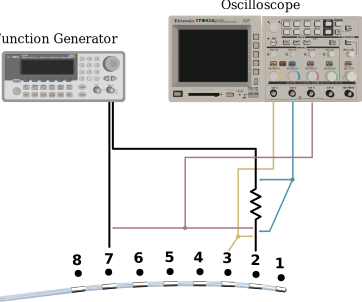
\includegraphics[scale=0.95]{content/pt2/08-InterfaceParameters/graphics/measurement_CPE_setup}
          \caption{\label{fig:pt2-measurement_CPE_setup}Diagram showing the measurement configuration used to measure the CPE response and interface series resistance.}
      \end{figure}
      By measuring the current through electrode two and the voltage across the interface (measured between electrodes two and three), the impedance of the interface is calculated.
      A diagram of the measurement setup is shown as \cref{fig:pt2-measurement_CPE_setup}.
      For each of the six solutions, twenty frequencies (log-spaced) were sampled between \SI{50}{\milli\hertz} and \SI{10}{\kilo\hertz} for the impedance measurements.
      At each frequency the stimulus waveform amplitude was re-adjusted to be \SI{300}{\milli\volt}-peak as the interface's impedance changed.
      \begin{figure}
        \centering
        \includegraphics{content/pt2/08-InterfaceParameters/graphics/displacement_impedanceVsFrequency_magnitude_thesis}
        \caption{\label{fig:pt2-graph_impedanceVsFrequency_magnitude}Impedance magnitude of both the measured interface response and the fitted response at each of the six concentrations of PBS.}
      \end{figure}
      \begin{figure}
        \centering
        \includegraphics{content/pt2/08-InterfaceParameters/graphics/displacement_impedanceVsFrequency_phase_thesis}
        \caption{\label{fig:pt2-graph_impedanceVsFrequency_phase}Impedance phase of both the measured interface response and the fitted response at each of the six concentrations of PBS.}
      \end{figure}
      \Cref{fig:pt2-graph_impedanceVsFrequency_magnitude,fig:pt2-graph_impedanceVsFrequency_phase} show the calculated impedance magnitude and phase from measurements as markers and simulation results from fitted parameters as traces.
      \begin{figure}[ht]
        \centering
        \includegraphics{content/pt2/08-InterfaceParameters/graphics/SpiceModel_opitimisation}
        \caption{\label{fig:pt2-spiceModel_optimisation}The SPICE model schematic used to find optimum values for parameters of the CPE and interface series resistance. Parameters for the resistor mesh are those determined previously.}
      \end{figure}
      \Cref{fig:pt2-spiceModel_optimisation} shows the SPICE model used to simulate parameter values for the CPE and $R_{s}$.
      Final values were found by minimising the difference between the simulated response and the measured response using a Python script.
      For each set of parameter values in the optimisation, the script builds a SPICE circuit based on the values, simulates the circuit, calculates the interface impedance and compares the values to the measured results.
      The process is automated and runs until a minimum error between simulated and measured results is found.
      Once found, the script exits and displays the final values of each parameter.

      After parameter values are found for each concentration of PBS, another optimisation is made to fit relevant parameters to PBS concentration.
      The parameters that scale with concentration are the series resistance ($R_{S}$) and the CPE's impedance magnitude at \SI{50}{\milli\hertz}.
      The final fit expresses these parameters as functions dependent on PBS concentration (equivalent to salinity).
      \begin{figure}
        \centering
        \includegraphics{content/pt2/08-InterfaceParameters/graphics/scalingFactors_Displacement_Thesis}
        \caption{\label{fig:pt2-scalingFactors_Displacement_Thesis}Plot showing fitted parameter values for the CPE impedance magnitude at \SI{50}{\milli\hertz} and series resistance at each of the six concentrations of PBS (shown as markers). The solid trace shows the resulting fit between those values as a function of concentration.}
      \end{figure}
      Individual parameter values for each concentration, along with the resulting fit, is shown in \cref{fig:pt2-scalingFactors_Displacement_Thesis}.
      % Measurements of the CPE's vertical position were made at \SI{50}{\milli\hertz}, as opposed to the parameters defined value at \SI{1}{\hertz}.
      Measurement of the vertical position of the CPE's impedance magnitude trace was made at \SI{50}{\milli\hertz} as opposed to the parameter's defined value of \SI{1}{\hertz}.
      This was done to avoid any effect from the series resistance interfering with the measured value.
      As the slope of the CPE is always the same (even between concentrations), the value can be easily converted back to the equivalent value at \SI{1}{\hertz}.
      Measured resistances at high frequencies include the inter-electrode resistance ($R_{23}$) which has been included in the plot, but is later subtracted to leave only $R_{S}$.
      \begin{table}
        \centering
        \begin{tabular}{r | l}
          Parameter & Value \\
          \hline
          $m$& 1.34\\
          $k$ & 1.773\\
          |Z| @ \SI{1}{\hertz} ($\Omega$)& $3284 \times concentration^{-0.158}$ \\
          $R_{S}$ ($\Omega$)& $13.38 \times concentration^{-0.8397}$
        \end{tabular}
        \caption{\label{tab:CPEparams}CPE and $R_{s}$ parameters. Concentration is relative to the stock solution of phosphate buffered saline.}
      \end{table}
      The final parameters for the CPE and $R_{S}$ are given in \cref{tab:CPEparams}.

      % Edit checkpoint 2015-09-19 10:35


    \subsection{Faradaic current}
      \label{sect:pt2-faradaicCurrent_PBS}

      \begin{figure}
        \centering
        \includegraphics{content/pt2/08-InterfaceParameters/graphics/measurement_Faradaic_setup_initial}
        \caption{\label{fig:pt2-measurement_Faradaic_setup_initial}Illustration of the cyclic voltammetry measurement configuration used to measure the response of the interface when driven into Faradaic conduction mode.}
      \end{figure}
      Using the same oscilloscope and function generator as the previous measurement, the oscilloscope was set to measure voltage between electrodes two and seven and the current through the current sense resistor (\cref{fig:pt2-measurement_Faradaic_setup_initial}).
      The function generator was set to produce a triangle wave stimulus, or linear ramp, also between electrodes two and seven.
      Electrical current associated with Faradaic reactions rises exponentially after a threshold electrode overpotential.
      The point at which the electrical current draw begins to move exponentially with increasing voltage represents the onset of the associated reaction.
      \begin{figure}
        \centering
        \includegraphics{content/pt2/08-InterfaceParameters/graphics/faradaicOnset-all-average}
        \caption{\label{fig:pt2-faradaic_measurement}Graph showing measured Faradaic response of each concentration of PBS to a linearly increasing voltage between electrodes two and seven.}
      \end{figure}

      \Cref{fig:pt2-faradaic_measurement} shows measured data where the Faradaic response is evident for each concentration.
      The repeatability of these measurements was low although care was taken to recreate the same conditions for each run.
      To try and improve the repeatability the following was tried:
      \begin{itemize}
        \item Maintaining a constant ambient temperature
        \item Cleaning the electrodes between each measurement using isopropyl alcohol
        \item Keeping the electrolyte moving at a constant velocity using a motorised stirrer
        \item Allowing the system to settle for periods of two hours between measurements
      \end{itemize}
      These steps did reduce variation, but by no means removed it.
      Sweeping the voltage at \SI{0.12}{\volt\per\second} was slow enough that results did not appear to be too distorted but fast enough that a measurement run could be completed quickly.
      Completing measurements quickly seemed important at the time as it was often the case that an artefact would show up during a measurement run, which initially appeared to have no obvious cause, and affect the remainder of the experiments.
      These artefacts would manifest themselves sometimes as a peak at a certain voltage, otherwise as distortions to the current/voltage trace.
      A key insight was realising that after the voltage across a pair of electrodes had been pushed into Faradaic region they then began to behave differently, even after being returned to lower stimulus voltages.
      In \cref{fig:pt2-faradaic_measurement} it is clear that each concentration has a different Faradaic response.
      This means that when the maximum voltage is applied to each of the solutions that the highest concentration is driven further into its Faradaic region than the rest.
      That in turn would create an artefact that would appear on the remaining traces (those of lower concentration), that would not have otherwise been there.
      The issue of artefact and dependence on sweep rate led me to find other ways of measuring Faradaic currents.

      % Edit checkpoint 2015-09-19 10:42

      \subsubsection*{Step based Faradaic measurements}

        \begin{figure}
          \centering
          \includegraphics{content/pt2/08-InterfaceParameters/graphics/graph_64s_stirred}
          \caption{\label{fig:pt2-faradaic_decay}Graph showing measured response of two interfaces to a multiple step responses. Vertical dotted lines indicate when in time the step occurred. Dotted traces show points in time after each response. Measurements are between electrodes two and seven on the Octrode submerged in 1X PBS.}
        \end{figure}

        A revealing measurement came from the use of the Agilent E5270B precision measurement mainframe, the same instrument used to measure the streaming potential cells (\cref{part:doubleLayersOnInsulators}).
        By increasing the voltage between the electrodes in discrete steps and recording the current over time it became clear that the CPE was having a large effect on the Faradaic measurements.
        \Cref{fig:pt2-faradaic_decay} shows three transitions in steps of \SI{50}{\milli\volt} occurring \SI{64}{\second} apart.
        Dotted traces link measurements made a set time after each transition, with the delay times indicated to the left of the graph.
        So for example, the top trace represents data that would be obtained if the settling time after each step was one second.
        It shows that the longer the settling time is, the lower the measured current - even though the response is the same.
        This graph shows the effect the CPE is having on measurement results, as well as the duration of time necessary for the transient response to settle in most instances.

        \begin{figure}
          \centering
          \includegraphics{content/pt2/08-InterfaceParameters/graphics/graph_CPE_currentVsTime_thesis}
          \caption{\label{fig:graph_CPE_currentVsTime}Graph showing CPE discharge curve after a step transition between each of voltage trace in increasing order. Measurements are between electrodes two and seven on the Octrode submerged in 1X PBS. A delay of 10 000 seconds elapsed between each step.}
        \end{figure}
        Subsequent measurements of CPE settling time show that a delay of \SI{64}{\second} between steps is adequate to allow the CPE voltage to settle.
        Those measurements are shown as \cref{fig:graph_CPE_currentVsTime}, with the \SI{64}{\second} window highlighted in grey.
        The dependence of the capacitance upon voltage or current is clearly visible by comparing the \SI{0.64}{\volt} trace to that of the \SI{1.04}{\volt}.
        This variation is most likely the change in capacitance (and series resistance) that Schwan published in 1968~\cite{Schwan1968}.

        \begin{figure}
          \centering
          \includegraphics{content/pt2/08-InterfaceParameters/graphics/graph_currentTimeFaradaicCPE_Stacked_Thesis}
          \caption{\label{fig:graph_currentTimeFaradaicCPE_Stacked_Thesis}Graph showing measurements of four concentrations of PBS as each is stepped from \SI{0.55}{\volt} to \SI{0.95}{\volt}. Measurements are between electrodes two and seven on the Octrode. A delay of 64 seconds elapsed between each step. Dotted traces connect current measurements taken \SI{10}{\second} after each step.}
        \end{figure}
        \Cref{fig:graph_currentTimeFaradaicCPE_Stacked_Thesis} shows measurements of four concentrations of PBS overliad on top of one another.
        This graph reveals that not only does the capacitance vary with applied voltage, as was shown in \cref{fig:graph_CPE_currentVsTime}, but also with concentration of PBS.
        A consequence of this is that not waiting long enough to sample the current gives the impression that a higher concentration of PBS results in larger Faradaic currents.
        This is shown by the dotted trace that is sampled \SI{10}{\second} after each step, which I believe is representative of results obtained using cyclic voltammetry methods.
        Importantly -- the settled current draw for each concentration is the same.
        Any separation between concentrations at the sixty-four second mark for each step appear to be unordered.

        \subsubsection*{Successful measurement of Faradaic current}
        \begin{figure}
          \centering
          \includegraphics{content/pt2/08-InterfaceParameters/graphics/graph_currentVoltage_logY_Thesis}
          \caption{\label{fig:graph_currentVoltage_logY_Thesis}Graph showing the electrical current draw associated with Faradaic reactions versus applied electrode overpotential. Measurements used the stepped method with a wait time of \SI{64}{\second} between transitions. Vertical bars mark the standard deviation of the final forty measurements before the following step.}
        \end{figure}
        \Cref{fig:graph_currentVoltage_logY_Thesis} shows the collected measurements of the electrical current due to Faradaic reactions using the stepped measurement method.
        Spread in the measurements at low voltages is due to noise in the measurement samples.
        There are three important observations that can be made from this graph:
        \begin{enumerate}
          % \item The effect saline concentration below \SI{0.9}{\volt} has little to no significance on the Faradaic current draw.
          \item The concentration of saline has no measurable impact upon the Faradaic reaction rate when the applied overpotential between a pair of electrodes is less than \SI{0.9}{\volt}.
          \item The concentration of saline is directly to related to the rate of Faradaic reactions when the applied overpotential between a pair of electrodes is more than \SI{1.05}{\volt}.
          \item Between \SI{0.9}{\volt} and \SI{1.05}{\volt} of overpotential between electrodes, each trace transitions to a mode of saline concentration dependence in reverse order of saline concentration.
        \end{enumerate}

        It appears that the change in behaviour between \SI{0.9}{\volt} and \SI{1.05}{\volt} is due to a transition to diffusion-controlled conduction between electrodes.
        I hypothesise that below \SI{0.9}{\volt} the charging of the CPE draws available ions to the electrode, creating a layer of high ionic concentration at the surface irrespective of that of the solution bulk.
        It is this layer that is consumed by the Faradaic reactions at a rate that increases exponentially with electrode overpotential.
        The effect of the bulk solution concentration while this layer exists is negligible until the point at which the layer is consumed faster than it can be replenished.
        At this point, and with increasing overpotential, Faradaic conduction is governed by diffusion of ions from the solution bulk into that layer.
        The rate at which those new ions diffuse into the layer is a function of the concentration, or abundance of ions available in the bulk.
        This explains the divergence of conduction with concentration between \SI{0.9}{\volt} and \SI{1.05}{\volt} and why there is no observable dependence on the bulk ion concentration beforehand.
        As Faradaic reactions are dangerous in an implanted setting, and therefore to be avoided, interest in Faradaic reactions lies in determining their onset.
        For the purpose of our model, it is sufficient to place a \SI{0.9}{\volt} limit across a pair of electrodes and proceed on the basis that Faradaic conduction is not affected by the saline concentration.

        \begin{figure}
          \centering
          \includegraphics{content/pt2/08-InterfaceParameters/graphics/graph_faradaic_currentVsTimeThesis}
          \caption{\label{fig:graph_faradaic_currentVsTimeThesis} Graph comparing measured Faradaic response of a pair of interfaces (1.0X PBS) to the simulated response using fitted parameter values for $i_0$ and $n$. Each spike is a step in electrode overpotential, with the steps shown in the following graph.}
        \end{figure}
        \begin{figure}
          \centering
          \includegraphics{content/pt2/08-InterfaceParameters/graphics/graph_faradaic_currentVsVoltageThesis}
          \caption{\label{fig:graph_faradaic_currentVsVoltageThesis} Graph comparing the measured settled electrical currents of Faradaic reactions (in 1.0X PBS) for a pair of interfaces to simulated final values using the fitted parameter values for $i_0$ and $n$.}
        \end{figure}
        Using the ``step and wait'' method to measure electrical currents associated with Faradaic conduction gave improved results, both in repeatability and expected response.
        \Cref{fig:graph_faradaic_currentVsTimeThesis,fig:graph_faradaic_currentVsVoltageThesis} show results using the 1.0X PBS solution, with other concentrations following the same pattern.
        In \cref{fig:graph_faradaic_currentVsTimeThesis} it can be seen that the simulated CPE does not follow the decay curve of the interface after each transition.
        Notice again how the capacitance is dependent on the electrode overpotential, but the CPE fails to capture that information.
        Final parameter values for the Faradaic currents (the diodes of the model) are given in \cref{tab:FaradaicParams}.

        \begin{table}
          \caption{Faradaic parameters}
          \label{tab:FaradaicParams}
          \begin{center}
            \begin{tabular}{r | l}
                Parameter & Value \\
                \hline
                $i0$ & $2.757\thinspace pA$\\
                $n$ & 1.36\\
            \end{tabular}
          \end{center}
        \end{table}


    \subsection{Final model}


      Parameter values for each of the model's components have been found.
      Collecting the parameters that describe the interface's impedance results in \cref{tab:ModelParameters}.
      This table excludes the parameters of the resistor network as they do not describe the interface itself.

      \begin{table}
        \caption{Determined interface parameters for the St. Jude Medical Octrode in phosphate buffered saline. The parameter $concentration$ refers to the dilution of PBS, e.g., 0.025 for a one-fortieth dilution to 1.0 for the stock PBS mixture.}
        \label{tab:ModelParameters}
        \begin{center}
          \begin{tabular}{r | l}
              Parameter & Value \\
              \hline

              $R_{S}$ ($\Omega$)& $13.38 \times concentration^{-0.8397}$ \\

              $m$& 1.34\\
              $k$ & 1.773\\
              |Z| @ \SI{1}{\hertz} ($\Omega$)& $3284 \times concentration^{-0.158}$ \\

              $i0$ & $2.757\thinspace pA$\\
              $n$ & 1.36\\
          \end{tabular}
        \end{center}
      \end{table}

      \begin{figure}
        \centering
        
\includegraphics{content/pt2/08-InterfaceParameters/graphics/interfaceSchematic_PBS_Solved}
        \caption{\label{fig:interfaceSchematic_PBS_Solved} Schematic of the electrode-electrolyte interface including parameter values for platinum and buffered saline.}
      \end{figure}

      % Edit checkpoint 2015-09-19 10:52

\section{Epidural Insertion into Live Sheep}
  \label{sect:sheep_measurements}


  \begin{figure}
    \centering
    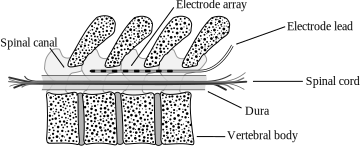
\includegraphics{content/pt2/08-InterfaceParameters/graphics/sheepSpine}
    \caption{\label{fig:sheepSpine} Diagram showing the positioning of the St. Jude Medical Octrode electrode array inside the sheep spinal cavity. The view is a cross-section of the spine with the dorsal side at the top.}
  \end{figure}

  The previous section dealt with measuring and fitting numerical values to the electrode-interface parameters in various solutions of buffered saline.
  Phosphate buffered saline, specifically a 0.1X concentration of a standard solution, was used for electrode characterisation as it was believed to be a good substitute for cerebrospinal fluid.
  Electronic engineers at Saluda Medical used these 0.1X PBS solutions to test their implant devices to make sure they were capable of driving and handling the impedance presented by the electrode-electrolyte interface and spinal cavity.
  Not knowing how closely the saline solutions resembled live biological spinal fluid they also tested their implants and electrodes in living sheep.
  A sheep's spinal canal is smaller than a human's, but large enough to insert an epidural electrode array, making them a relatively accessible means of in-vivo testing for medical applications.
  Geometrically they are similar enough for the sheep to be used as a test substitute for human spinal implant testing.
  Measurement in a live sheep's spinal canal still requires a lot of resources such as a surgeon, access to an operating theatre, equipment suitable for use in an operating theatre, ethical approval, and time.
  When experimenting with sheep, the sheep would be anaesthetised and kept alive for the duration of the experiments, which often last over twelve hours.
  A veterinary surgeon would prepare and monitor the sheep constantly during the experiments to ensure that it was fully anaesthetised and then euthanise the sheep at the end of testing.

  These tests offered an opportunity for me to characterise the electrode-electrolyte interface inside a living mammal.
  This section repeats the measurements and parameter value determination of the previous section but this time inside a living sheep's spinal cavity.
  The same electrode as was used in the previous measurements (St. Jude Medical Octrode) was inserted into the spinal cavity of the sheep (just outside the dura) for each experiment, as shown in \cref{fig:sheepSpine}.

  Sheep used to gather experimental data here were provided by the Keams Facility at the Royal North Shore Hospital of Sydney under the Animal Care and Ethics Committee approval.
  \label{edit:newSentence}Two sheep were used to gather measurement data, but inadequate electrode placement and a loss of spinal fluid from previous experiments meant that useful data was only obtained from the second sheep.
  These experiments complied with the Australian Code of Practice for the Care and Use of Animals for Scientific Purposes.
  In each case the sheep were injected with alfaxalone to induce anaesthesia and were then intubated and ventilated with an oxygen-air mixture containing isoflurane.
  During the course of experimentation the animals were monitored using electrocardiogram, arterial blood pressure, arterial saturation, and end-tidal (exhaled) carbon dioxide levels.
  All ethical considerations and procedures around animal testing were handled by Saluda Medical.
  Unless otherwise stated, measurement procedures and the equipment used in the hospital are the same as those used to measure the electrode-electrolyte response in PBS.

  \subsection{Inter-electrode resistivity}

    Trans-impedance measurements were the first to be made once the electrode array was inserted into the sheep's spinal canal.
    These measurements were more extensive than those made in saline as additional stimulus electrode pairs were used.
    The extra measurements were made with the hope that they may capture more information regarding the impedance structure of the surrounding spine geometry; mostly the bone.

    \begin{figure}
      \centering
      \includegraphics{content/pt2/08-InterfaceParameters/graphics/sheep_transimpedance_doubleFit_mag_thesis}
      \caption{\label{fig:sheep_transimpedance_doubleFit_mag} Graph showing measured and simulated trans-impedance magnitudes for twenty five combinations of stimulus-measure pairs of electrodes.}
    \end{figure}

    \begin{figure}
      \centering
      \includegraphics{content/pt2/08-InterfaceParameters/graphics/sheep_transimpedance_doubleFit_phase_thesis}
      \caption{\label{fig:sheep_transimpedance_doubleFit_phase} Graph showing measured and simulated trans-impedance phase for twenty five combinations of stimulus-measure pairs of electrodes.}
    \end{figure}

    \Cref{fig:sheep_transimpedance_doubleFit_mag,fig:sheep_transimpedance_doubleFit_phase} show both the measured and simulated results for the impedance magnitude and phase response respectively.
    The magnitude measurements show that when stimulating between electrodes one and eight and measuring on electrodes two and three that the impedance is approximately that of the one-tenth concentration of PBS (compared with results from \cref{fig:pt2-graph_transimpedance_pbs}).
    This result appears to support the idea that a one-tenth concentration of a standard buffered saline solution is a good substitute for a spinal cavity.
    For the case where the stimulus is placed between electrode one and two and the impedance is measured between electrodes seven and eight, the comparison suggests a lower concentration of PBS than 1/10\textsuperscript{th}.
    Swapping the stimulus and measure electrodes around gave different trans-impedance values, i.e., the point at 12,78 does not equal that of 78,12.
    This suggests that the electrode array shifted inside the cavity over the course of the measurements.

    One important insight from these measurements is the phase response, as is shown in \cref{fig:sheep_transimpedance_doubleFit_phase}.
    As much as 30 degrees of phase angle between the stimulus current and electrode voltage was observed when separation between the stimulus and measure pairs is at its maximum.
    This shows that the spinal cavity itself is a significantly reactive component.
    For comparison, the PBS solutions displayed no measurable reactance for all of the equivalent trans-impedance measurements.
    The decreasing phase angle of measurements using one and eight as stimulus electrodes is a result of the measured pair of electrodes being between the stimulus, i.e., it is a result of our electrode choices.
    There are other instances where the phase angle appears to drop below zero, but these are likely an artefact of the measurements themselves.
    Those situations only occur when the stimulus and measured electrodes are adjacent to one another.
    This means the impedance, and therefore signal-to-noise ratio, was at its lowest.
    Stimulus current was reduced for the in-vivo measurements to prevent muscle spasms.

    \begin{table}
      \centering
      \begin{tabular}{r | l}
        Parameter & Value \\
        \hline
        $R_{eri}$ ($\Omega$)& 500\\
        $R_{sri}$ ($\Omega$)& 375\\
        $R_{li}$ ($\Omega$)& 176\\
        Depth (layers) & 5 \\
        Padding (layers) & 3 \\
      \end{tabular}
      \caption{\label{tab:RESparams_sheep} Determined resistor mesh parameters for an electrode array in a live sheep's spinal cavity.}
    \end{table}
    The simulated results shown in \cref{fig:sheep_transimpedance_doubleFit_mag,fig:sheep_transimpedance_doubleFit_phase} (shown as the red trace) were calculated using the resistor mesh parameter values shown in \cref{tab:RESparams_sheep}.
    Those values were determined using the same SciPy optimisation library for Python as was used to fit the values in PBS.

    % Edit checkpoint 2015-09-19 14:20


  \subsection{Constant phase \& series resistance}

    \begin{figure}
      \centering
      \includegraphics{content/pt2/08-InterfaceParameters/graphics/graph_Day2_Sheep_CPE_ImpedanceMagnitude}
      \caption{\label{fig:graph_Day2_Sheep_CPE_ImpedanceMagnitude} Graph showing measured CPE impedance magnitude response before and after termination.}
    \end{figure}

    \begin{figure}
      \centering
      \includegraphics{content/pt2/08-InterfaceParameters/graphics/graph_Day2_Sheep_CPE_ImpedancePhase}
      \caption{\label{fig:graph_Day2_Sheep_CPE_ImpedancePhase} Graph showing measured CPE impedance phase response before and after termination.}
    \end{figure}


    \Cref{fig:graph_Day2_Sheep_CPE_ImpedanceMagnitude,fig:graph_Day2_Sheep_CPE_ImpedancePhase} show impedance magnitude and the phase response of the CPE at the interface between the electrode and the sheep's spinal cavity.
    Measurements were made over a thirty minute period starting two minutes before termination.

    An important question I hoped to answer was whether the impedance response in live sheep would be any different to that of a dead sheep.
    Results indicate that there is practically no difference for at least thirty minutes after termination.
    Measurements should have been carried out over a longer time-frame after termination as it would likely take longer for the fluid composition to change.
    As the measurements required termination of the sheep, they had to be done after all other experiments had been completed.
    Since each sheep was shared between other research groups this meant that termination happened late (early the following morning) due to accumulated delays in previous experiments.
    Measuring the CPE response in the spinal cavity of a butchered sheep would offer a useful reference point for those measurements.


    \begin{figure}
      \centering
      \includegraphics{content/pt2/08-InterfaceParameters/graphics/graph_displacement-withSheep_impedanceVsFrequency_magnitude_thesis}
      \caption{\label{fig:graph_displacement-withSheep_impedanceVsFrequensy_magnitude} Graph showing average CPE response in live sheep compared to the six solutions of PBS, visible as the grey traces, and simulated response based on fitted parameters.}
    \end{figure}

    \begin{figure}
      \centering
      \includegraphics{content/pt2/08-InterfaceParameters/graphics/graph_displacement-withSheep_impedanceVsFrequency_phase_thesis}
      \caption{\label{fig:graph_displacement-withSheep_impedanceVsFrequency_phase} Graph showing average CPE response in a live sheep's spinal cavity compared to six concentrations of PBS, visible as grey traces, and simulated response based on fitted parameters.}
    \end{figure}

    \Cref{fig:graph_displacement-withSheep_impedanceVsFrequensy_magnitude,fig:graph_displacement-withSheep_impedanceVsFrequency_phase} compare the average impedance (both magnitude and phase) of the previous graphs with the six concentrations of PBS used in the previous section.
    Simulated results from a numerical fit to the measured data appear as the red trace.
    At low frequencies, below \SI{1}{\hertz}, the simulated data deviates substantially from measured results.
    The cause for this is unclear, but in \cref{chap:fluid_mimicry} the opposite response appears when using unbuffered saline solutions - which may provide a clue.
    What is interesting is that the series resistance in sheep spine is similar to that of a 0.25X PBS solution, whereas the CPE behaves more like that of a concentration much lower than 0.025X.
    Based on this data, a one-tenth concentration of PBS does appear to make a reasonable trade-off between the CPE and series resistance parts, but the match between both is poor.
    In the following section the possibility of creating a solution that better matches these results will be explored.


  \subsection{Faradaic current}

    Faradaic measurements on the live animal were abandoned as they were deemed likely to cause muscle contractions by the veterinarian surgeon.
    Attempts were made to measure Faradaic response using a much lower stimulus current but no signal was evident above the noise so were discarded.
    These measurements may be possible if done long enough post-termination so as not to cause muscle movement.

  \subsection{Final model}

    \begin{table}
      \caption{Determined interface parameters for the electrode array in a live sheep's spinal cavity.}
      \label{tab:ModelParameters_sheep}
      \begin{center}
        \begin{tabular}{r | l}
            Parameter & Value \\
            \hline

            $R_{S}$ & \SI{126}{\ohm} \\

            $m$& 1.34\\
            $k$ & 1.77\\
            |Z| @ \SI{1}{\hertz} ($\Omega$)& \SI{11.3}{\kilo\ohm} \\

            $i0$ & Undetermined\\
            $n$ & Undetermined\\
        \end{tabular}
      \end{center}
    \end{table}
    Parameter values for the final sheep model are presented in \cref{tab:ModelParameters_sheep}.
    Unfortunately, the diode/Faradaic parameters were not obtained on live sheep due to concerns of causing violent muscle contractions.
    Those measurements are likely to be of value to implant designers as they provide a reference for the beginnings of Faradaic conduction.
    Access to an recently terminated sheep's spine, and a surgeon, would provide a way of collecting those Faradaic measurements and additional post-termination samples.

    Parameters for the interface model in sheep have been fitted.
    It appears as though buffered saline, of any concentration, is not an ideal representation of a live sheep's spinal cavity.
    The next research question is to determine if it is possible to create a solution that better matches those impedance characteristics.

    % Edit checkpoint 2015-09-19 14:33